% In Z[i], b = 2+i is a universal side divisor: every blue point is at
% distance exactly 1 from a multiple r·(2+i) (arrows), and red points are
% exact multiples.
% Source: book/tex/H113/ring-flavors.tex (§ When is a ring a Euclidean domain?).
\documentclass[border=2mm]{standalone}
\usepackage{tikz}
\usetikzlibrary{arrows.meta}
\begin{document}
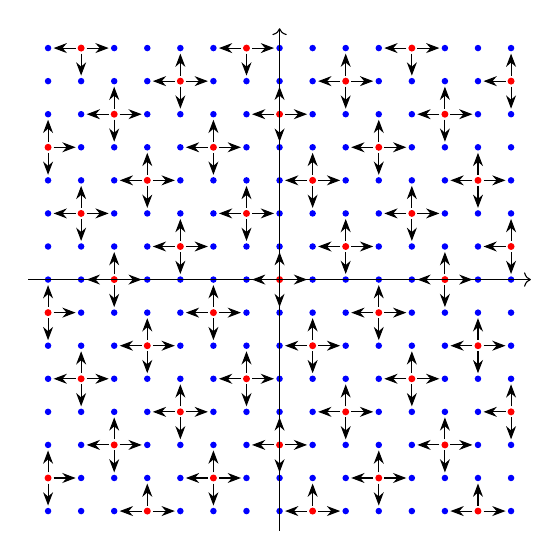
\begin{tikzpicture}[scale=0.42]
  \foreach \x in {-7,...,7}{
    \foreach \y in {-7,...,7}{
      \pgfmathtruncatemacro{\rre}{round((2*\x+\y)/5)}
      \pgfmathtruncatemacro{\rim}{round((2*\y-\x)/5)}
      \pgfmathsetmacro{\bx}{2*\rre-\rim}
      \pgfmathsetmacro{\by}{\rre+2*\rim}
      \pgfmathsetmacro{\dist}{veclen(\x-\bx,\y-\by)}
      \pgfmathtruncatemacro{\side}{(\dist>0.99 && \dist<1.01)?1:0}
      \pgfmathtruncatemacro{\inrange}{(\bx>-7.5 && \bx<7.5 && \by>-7.5 && \by<7.5)?1:0}
      \ifnum\side=1
        \fill[blue] (\x,\y) circle (2.8pt);
        \ifnum\inrange=1
          \draw[-{Stealth}, shorten >=2pt, shorten <=2pt] (\bx,\by) -- (\x,\y);
        \fi
      \fi
      \pgfmathtruncatemacro{\exact}{(\dist<0.01)?1:0}
      \ifnum\exact=1 \fill[red] (\x,\y) circle (3pt); \fi
    }
  }
  \draw[->] (-7.6,0) -- (7.6,0);
  \draw[->] (0,-7.6) -- (0,7.6);
\end{tikzpicture}
\end{document}
